
% This is "sig-alternate.tex" V2.0 May 2012
% This file should be compiled with V2.5 of "sig-alternate.cls" May 2012
%
% This example file demonstrates the use of the 'sig-alternate.cls'
% V2.5 LaTeX2e document class file. It is for those submitting
% articles to ACM Conference Proceedings WHO DO NOT WISH TO
% STRICTLY ADHERE TO THE SIGS (PUBS-BOARD-ENDORSED) STYLE.
% The 'sig-alternate.cls' file will produce a similar-looking,
% albeit, 'tighter' paper resulting in, invariably, fewer pages.
%
% ----------------------------------------------------------------------------------------------------------------
% This .tex file (and associated .cls V2.5) produces:
%       1) The Permission Statement
%       2) The Conference (location) Info information
%       3) The Copyright Line with ACM data
%       4) NO page numbers
%
% as against the acm_proc_article-sp.cls file which
% DOES NOT produce 1) thru' 3) above.
%
% Using 'sig-alternate.cls' you have control, however, from within
% the source .tex file, over both the CopyrightYear
% (defaulted to 200X) and the ACM Copyright Data
% (defaulted to X-XXXXX-XX-X/XX/XX).
% e.g.
% \CopyrightYear{2007} will cause 2007 to appear in the copyright line.
% \crdata{0-12345-67-8/90/12} will cause 0-12345-67-8/90/12 to appear in the copyright line.
%
% ---------------------------------------------------------------------------------------------------------------
% This .tex source is an example which *does* use
% the .bib file (from which the .bbl file % is produced).
% REMEMBER HOWEVER: After having produced the .bbl file,
% and prior to final submission, you *NEED* to 'insert'
% your .bbl file into your source .tex file so as to provide
% ONE 'self-contained' source file.
%
% ================= IF YOU HAVE QUESTIONS =======================
% Questions regarding the SIGS styles, SIGS policies and
% procedures, Conferences etc. should be sent to
% Adrienne Griscti (griscti@acm.org)
%
% Technical questions _only_ to
% Gerald Murray (murray@hq.acm.org)
% ===============================================================
%
% For tracking purposes - this is V2.0 - May 2012

\documentclass{sig-alternate}

\usepackage{cite}
\usepackage{dblfloatfix}
\usepackage{setspace}
\usepackage{multirow}
\usepackage{array}
\usepackage{import}
\usepackage{tikz}
\usepackage[bookmarks=false]{hyperref}
\usepackage[hyphenbreaks]{breakurl}
\usepackage{graphicx}
\usepackage{xcolor,colortbl}
\usepackage{tabularx}
\usepackage{flushend}
\usepackage{amsmath}
\usepackage{subcaption}

\begin{document}
%
% --- Author Metadata here ---
\conferenceinfo{WWW}{'16 Montereal, Canada}
%\CopyrightYear{2007} % Allows default copyright year (20XX) to be over-ridden - IF NEED BE.
%\crdata{0-12345-67-8/90/01}  % Allows default copyright data (0-89791-88-6/97/05) to be over-ridden - IF NEED BE.
% --- End of Author Metadata ---

\title{Adoption and evolution of social networks from a cohort perspective}

%\title{Alternate {\ttlit ACM} SIG Proceedings Paper in LaTeX
%Format\titlenote{(Produces the permission block, and
%copyright information). For use with
%SIG-ALTERNATE.CLS. Supported by ACM.}}
%\subtitle{[Extended Abstract]
%\titlenote{A full version of this paper is available as
%\textit{Author's Guide to Preparing ACM SIG Proceedings Using
%\LaTeX$2_\epsilon$\ and BibTeX} at
%\texttt{www.acm.org/eaddress.htm}}}
%
% You need the command \numberofauthors to handle the 'placement
% and alignment' of the authors beneath the title.
%
% For aesthetic reasons, we recommend 'three authors at a time'
% i.e. three 'name/affiliation blocks' be placed beneath the title.
%
% NOTE: You are NOT restricted in how many 'rows' of
% "name/affiliations" may appear. We just ask that you restrict
% the number of 'columns' to three.
%
% Because of the available 'opening page real-estate'
% we ask you to refrain from putting more than six authors
% (two rows with three columns) beneath the article title.
% More than six makes the first-page appear very cluttered indeed.
%
% Use the \alignauthor commands to handle the names
% and affiliations for an 'aesthetic maximum' of six authors.
% Add names, affiliations, addresses for
% the seventh etc. author(s) as the argument for the
% \additionalauthors command.
% These 'additional authors' will be output/set for you
% without further effort on your part as the last section in
% the body of your article BEFORE References or any Appendices.

\numberofauthors{4} %  in this sample file, there are a *total*
% of EIGHT authors. SIX appear on the 'first-page' (for formatting
% reasons) and the remaining two appear in the \additionalauthors section.
%
\author{
% You can go ahead and credit any number of authors here,
% e.g. one 'row of three' or two rows (consisting of one row of three
% and a second row of one, two or three).
%
% The command \alignauthor (no curly braces needed) should
% precede each author name, affiliation/snail-mail address and
% e-mail address. Additionally, tag each line of
% affiliation/address with \affaddr, and tag the
% e-mail address with \email.
%
% 1st. author
\alignauthor
Samuel Barbosa\\
       \affaddr{Institute of Mathematics and Statistics}\\
       \affaddr{University of S\~ao Paulo}\\
       \affaddr{S\~ao Paulo, Brazil}\\
       \email{sam@ime.usp.br}
 %2nd. author
\alignauthor
Dan Cosley\\
       \affaddr{Department of Information Science}\\
       \affaddr{Cornell University}\\
       \affaddr{Ithaca, NY 14853 USA}\\
       \email{danco@cs.cornell.edu}
 %3rd. author
\alignauthor
Amit Sharma\\
       \affaddr{Microsoft Research}\\
       \affaddr{New York, NY 10011 USA}\\
       \email{amshar@microsoft.com}
 %4th. author
\and
\alignauthor
Roberto M. Cesar-Jr\\
       \affaddr{Institute of Mathematics and Statistics}\\
       \affaddr{University of S\~ao Paulo}\\
       \affaddr{S\~ao Paulo, Brazil}\\
       \email{cesar@ime.usp.br}
}
% There's nothing stopping you putting the seventh, eighth, etc.
% author on the opening page (as the 'third row') but we ask,
% for aesthetic reasons that you place these 'additional authors'
% in the \additional authors block, viz.
%\additionalauthors{Additional authors: John Smith (The Th{\o}rv{\"a}ld Group,
%email: {\texttt{jsmith@affiliation.org}}) and Julius P.~Kumquat
%(The Kumquat Consortium, email: {\texttt{jpkumquat@consortium.net}}).}

\date{10 October 2015}
% Just remember to make sure that the TOTAL number of authors
% is the number that will appear on the first page PLUS the
% number that will appear in the \additionalauthors section.

\maketitle
\begin{abstract}
Online communities provide a fertile ground for analyzing people's behavior and improving our understanding of social processes. However, like any complex social system, the key part is detail in identifying and accounting for underlying heterogeneity and selection effects among people in these communities. Using Reddit as an example community, we study the evolution of users based on comments and submissions data from 2007 to 2014, creating a cohort of users who join each year. Even with one of the simplest sources of differentiation between users---their age in the community---we find wide differences in people's behavior, including comment activity, effort and survival, both within cohorts and with the averages over the whole community. Not controlling for these variations may not only dilute the overall effects that we observe, but in some cases, it can lead us to the wrong conclusions (Simpson's paradox).  These observations can be puzzling: for instance, we observe that average comment length decreases over any fixed period of time, but comment length in each cohort of users steadily increases during the same period after an abrupt initial drop. Finally, we analyze subcommunities on Reddit through the same lens of age and we find an enormous first-mover advantage: subreddits created early in the community's history are orders of magnitude more active than even successful subreddits created later, even among cohorts of users who join much later.
\end{abstract}

%% DC 10: Need to catch these.
We need categories, terms, and keywords

user behavior
cohort
reddit

% A category with the (minimum) three required fields
%\category{H.4}{Information Systems Applications}{Miscellaneous}
%A category including the fourth, optional field follows...
%\category{D.2.8}{Software Engineering}{Metrics}[complexity measures, performance measures]
%\terms{Theory}
%\keywords{ACM proceedings, \LaTeX, text tagging}

\section{Introduction}

%% DC 10: After seeing this I'm less convinced it was a good idea for me to suggest it, at least as an introduction.  It might read/work better as a related work section now, assuming that we have the previous work available to cite.  
In previous work, researchers have studied the relationship of different cohorts adopting new technologies and how users that did not grow in a technological environment show different characteristics when compared with the younger generations. This external variable to the social network might explain many different aspects of how adoption of a network happens. Just as users experience outside the network vary according to their age and influence their behavior, users' experience inside the network throughout time vary as the network evolves. Users in the early stages of a social network have a very different experience from latter users.

\textbf{\textit{Are users evolving in different ways based on when they join the network? How is an early user different from a late user?}}

Evolution in this sense can be interpreted in many different ways. Researchers have looked into many aspects of how user behavior change, how frequent they post, how users adopt new language, how likely a user is to survive in the network (which is also related with the problem of predicting which users are going to depart from your network). Based on this, we have to understand what we are looking for in the user behavior.

%% DC 10: This really isn't a separate question; these are common kinds of questions that realted work might ask
\textbf{\textit{What can ``different'' be? Effort, activity, survival?}}

This evolving process of users changing inside of the network change the network itself. We know that the idea users have from a social network might change their willingness to try it, just as we know how the initial experience might impact in the user future behavior \cite{Miller2015}. But the community evolving in itself changes the idea users outside have about it \cite{Danescu-niculescu-mizil2013}. This internal evolution together with the novelty that the influx of users bring make reddit a very interesting evironment to understand, for sub-communities known as subreddits as being created all the time and in different contexts, which raises the following question.

\textbf{\textit{Are communities evolving in different ways based on when they are created in the network?}}

%% DC 10: Problem. https://www.reddit.com/wiki/reddit_101 new users are subscribed by default to a number of subreddits, which I'm guessing explains an enormous amount of the advantage of reddits from 2008.  That makes this part much less interesting for us to talk about.  See if these subreddits were created mostly in 2008. http://i.imgur.com/4PxSX4e.png (and also, how this list has changed over time).
%%
%% DC 10: There's a reasonable chance there's still a fun paper just about users, but what we don't want to do is say that our cohort analysis really bought us something that would have been better bought by actually looking at site norms.

%% We can check weather the introduction or removal of subreddits in the default set influences significantly activity in them. Since the default are chosen based on the activity on them to begin with, it is more a positive reinforcement than a decisive bias for the community (as we can see, subreddits that are not ``doing well'' are removed, there is more on the comments in https://www.reddit.com/r/defaults). Even though, it might be worth to remove the subreddit section. We could also anlize wheather or not being included or removed from the default changes something for the community.
\begin{table}[htbp]
\centering
\tabcolsep=0.11cm
\singlespacing
\fontsize{7pt}{8pt}\selectfont
\begin{tabular}{|>{\raggedright\centering\arraybackslash}m{1.5cm}|m{6.8cm}|}
\hline
December 31, 2009 & announcements, AskReddit, blog, funny, gaming, pics, politics, programming, reddit.com, science, worldnews, WTF \\ \hline
October 18, 2011 & AdviceAnimals, Announcements, AskReddit, AskScience, Atheism, Aww, BestOf, Blog, Funny, Gaming, IamA, Movies, Music, Pics, Politics, Science, Technology, TodayILearned, Videos, WorldNews, WTF \\ \hline
October 19, 2012 & AdviceAnimals, Announcements, AskReddit, Aww, BestOf, Blog, Funny, Gaming, IamA, Movies, Music, News, Pics, Science, Technology, TodayILearned, Videos, WorldNews, WTF, Gifs, Television, Explainlikeimfive, Earthporn, books, AskScience \\ \hline
July 17, 2013 & AdviceAnimals, AskReddit, Aww, BestOf, Books, EarthPorn, ExplainLikeImFive, Funny, Gaming, Gifs, IAmA, Movies, Music, News, Pics, Science, Technology, Television, TodayILearned, Videos, WorldNews, WTF \\ \hline
January 1, 2014 & AdviceAnimals, AskReddit, AskScience, Aww, BestOf, Books, EarthPorn, ExplainLikeImFive, Funny, Futurology, Gaming, Gifs, IAmA, Movies, Music, News, Pics, Science, Sports, Technology, Television, TodayILearned, Videos, WorldNews \\ \hline
April 19, 2014 & AdviceAnimals, AskReddit, AskScience, Aww, BestOf, Books, EarthPorn, ExplainLikeImFive, Funny, Gaming, Gifs, IAmA, Movies, Music, News, Pics, Science, Sports, Television, TodayILearned, Videos, WorldNews \\ \hline
May 7, 2014 & announcements, Art, AskReddit, askscience, aww, blog, books, creepy, dataisbeautiful, DIY, Documentaries, EarthPorn, explainlikeimfive, Fitness, food, funny, Futurology, gadgets, gaming, GetMotivated, gifs, history, IAmA, InternetIsBeautiful, Jokes, LifeProTips, listentothis, mildlyinteresting, movies, Music, news, nosleep, nottheonion, oldschoolcool, personalfinance, philosophy, photoshopbattles, pics, science, Showerthoughts, space, sports, television, tifu, todayilearned, TwoXChromosomes, UpliftingNews, videos, worldnews, writingprompts \\ \hline
\end{tabular}
\caption{Default subrredits over time.}
\end{table}

\begin{table}[htbp]
\centering
\tabcolsep=0.11cm
\singlespacing
\fontsize{7pt}{8pt}\selectfont
\begin{tabular}{|>{\raggedright\centering\arraybackslash}m{1.5cm}|c|c|c|c|c|c|c|c|}
\hline
 & 2007 & 2008 & 2009 & 2010 & 2011 & 2012 & 2013 & 2014 \\ \hline
December 31, 2009 & 5 & 6 & 1 & - & - & - & - & - \\ \hline
October 18, 2011 & 3 & 14 & 2 & 2 & - & - & - & - \\ \hline
October 19, 2012 & 2 & 16 & 3 & 2 & 2 & - & - & - \\ \hline
July 17, 2013 & 2 & 15 & 2 & 1 & 2 & - & - & - \\ \hline
January 1, 2014 & 3 & 14 & 2 & 2 & 3 & - & - & - \\ \hline
April 19, 2014 & 3 & 13 & 2 & 2 & 2 & - & - & - \\ \hline
May 7, 2014 & 4 & 23 & 6 & 5 & 4 & 7 & 1 & - \\ \hline
\end{tabular}
\caption{Count of subreddits per creation year for each default set of.}
\end{table}

Kooti et al. \cite{Kooti2010} showed that social conventions can define the evolution of a community and the early adopters play a major role in designing these conventions, even if at the time this is not known by them. Evidence for the need of a retweeting mechanism in Twitter was evident in the early stages of the community and, out of the many possibilities that coexisted, the ``RT'' tag survived. Early adopters of these conventions are core users, well connected and presenting high activity. Just as Twitter, reddit network evolved from a relatively small set of users and subreddits. Wheather or not these early adopter of reddit laid the foundations in terms of content and behavior is not necessarily clear. It is reasonable to imagine that users would always look for content in subreddits that were created around the time they joined the network, for they might refer to the current context they are inserted into. Therefore, we propose the following question.

\textbf{\textit{Is there a consolidation point in a social network where the ``core content'' is established? Can this core change over time?}}

User-Network homophily? They connect because they are similar or do they become similar as the user evolves? Are the ``dissimilar'' leaving?
Looking at how reddit looked like at a particular point in time is a different question from how users evolve, and much of the user evolution depends on the environment a user finds when they first join the network. In many ways, this is an initial value problem, but separating what is due to the evolution of the network and what comes from the different demographics outside the network is not always clear.

\textbf{\textit{Are latter users intrinsically different from earlier users or are they having different initial experiences?}}

\section{Time matters}  %% DC 12: Bad pun (matters = important, matters = specifics)

%% DC 12: Okay, taking a new stab at an outline/argument for this that better fits the introduction, which is much more about time than it was.  
%% I do not and will not have time to write this up, but I think a lot of it will be pretty straightforward.  I'm hoping that Sam sees it as reasonable tonight, and that he tonight and/or Amit tomorrow can fill in a good amount of this and change/tweak things as you see that they work or don't.
%% Cites in this section don't _all_ have to be about modeling user behavior in online communities, but we want to make sure that's embedded in the story wherever possible.

\subsection{Why accounting for time is important}

Why time is important: the incoming users and community both likely change over time.  
Differences in cohorts \cite{Welser2011a}

Users 1: The user adoption curve means that enthusiasts likely join earlier.  
Self-selection \cite{Li2008}, 

Users 2: Overall patterns of use might change because the overall population of internet users is still changing (this `would be a place to critique the Mexican desensitization to violence paper).

Community 1: The nature or goals of the community can change.  Flixter.  Digg.  Reddit iteself has a number of subcommunities that are the default set for new users---and they change over time. 

Community 2: Successful communities often grow very rapidly, providing more content to react to (which is both good and bad -- there's more to interact with, but getting responses might be a lot easier in a small than large community) and new challenges for management (Wikipedia policies).  

Community 3: Behavior within the community changes as new users come.  Conventions are created.  Language changes.  And, people likely model what they see. 

Pithy summary of why time is important from the above.

\subsection{Accounting for time and change}

Using ordinal time when timestamps aren't available or are coarse. (Cosley et al. Suri paper from 2010 about ordinal time; k-exposure; must be others).  We're more interested in the general case when time data is available.  

Statistical tools: Using joining time as a predictor/control variable (e.g., in regressions).  (Find examples).  
More sophisticated time series analysis.  But, we're more interested in simpler analyses and effective ways to visualize behavior.
%% DC 12: This idea of effective visualizations of behavior could be a framing of the whole paper in some worlds, although it's probably a little late to move in that direction and would require us to become more expert in visualization. 

Adjusting time relative to phenomena or events of interest.  Normalizing clock times to local time (Macy and Golder twitter paper) or internal clock time (Liz paper under submission to CHI).  Normalizing to an event of interest (e.g., Crandall paper 'first interaction' in Wikipedia).  

Using cohorts.  (Find examples.)
\cite{Welser2011a}

%% DC 12: I was going to have this as the first subsection, but the flow worked better to start with time.  So, then I went to put it as the third subsection, but I think a lot of the specifics that would have been here will come up in the discussion of time.  So now I don't think this needs to be here.  There are some worlds that it comes as part of the Reddit subsection, but I think the most likely outcome now is that at the beginning of the analysis, there's a brief section that introduces that we're going after these questions, and then at the beginning of each analysis we point to enough related work to help illustrate that it's an important question, to help us define it in Reddit, and (ideally) to charcterize whether other work on that question has done some of this work around accounting for time.
% \subsection{Modeling user effort in online communities}


%In previous work, researchers have studied the relationship of different cohorts adopting new technologies and how users that did not grow in a technological environment show different characteristics when compared with the younger generations. This external variable to the social network might explain many different aspects of how adoption of a network happens. Just as users experience outside the network vary according to their age and influence their behavior, users' experience inside the network throughout time vary as the network evolves. Users in the early stages of a social network have a very different experience from latter users.

%\textbf{\textit{Are users evolving in different ways based on when they join the network? How is an early user different from a late user?}}

%Evolution in this sense can be interpreted in many different ways. Researchers have looked into many aspects of how user behavior change, how frequent they post, how users adopt new language, how likely a user is to survive in the network (which is also related with the problem of predicting which users are going to depart from your network). Based on this, we have to understand what we are looking for in the user behavior.

%% DC 10: This really isn't a separate question; these are common kinds of questions that realted work might ask
\textbf{\textit{What can ``different'' be? Effort, activity, survival?}}

%This evolving process of users changing inside of the network change the network itself. We know that the idea users have from a social network might change their willingness to try it, just as we know how the initial experience might impact in the user future behavior \cite{Miller2015}. But the community evolving in itself changes the idea users outside have about it \cite{Danescu-niculescu-mizil2013}. This internal evolution together with the novelty that the influx of users bring make reddit a very interesting evironment to understand, for sub-communities known as subreddits as being created all the time and in different contexts, which raises the following question.

\textbf{\textit{Are communities evolving in different ways based on when they are created in the network?}}

%% DC 10: Problem. https://www.reddit.com/wiki/reddit_101 new users are subscribed by default to a number of subreddits, which I'm guessing explains an enormous amount of the advantage of reddits from 2008.  That makes this part much less interesting for us to talk about.  See if these subreddits were created mostly in 2008. http://i.imgur.com/4PxSX4e.png (and also, how this list has changed over time).
%%
%% DC 10: There's a reasonable chance there's still a fun paper just about users, but what we don't want to do is say that our cohort analysis really bought us something that would have been better bought by actually looking at site norms.

%% Sam 10: We can check weather the introduction or removal of subreddits in the default set influences significantly activity in them. Since the default are chosen based on the activity on them to begin with, it is more a positive reinforcement than a decisive bias for the community (as we can see, subreddits that are not ``doing well'' are removed, there is more on the comments in https://www.reddit.com/r/defaults). Even though, it might be worth to remove the subreddit section. We could also analyze wheather or not being included or removed from the default changes something for the community.
%\begin{table}[htbp]
%\centering
%\tabcolsep=0.11cm
%\singlespacing
%\fontsize{7pt}{8pt}\selectfont
%\begin{tabular}{|>{\raggedright\centering\arraybackslash}m{1.5cm}|m{6.8cm}|}
%\hline
%December 31, 2009 & announcements, AskReddit, blog, funny, gaming, pics, politics, programming, reddit.com, science, worldnews, WTF \\ \hline
%October 18, 2011 & AdviceAnimals, Announcements, AskReddit, AskScience, Atheism, Aww, BestOf, Blog, Funny, Gaming, IamA, Movies, Music, Pics, Politics, Science, Technology, TodayILearned, Videos, WorldNews, WTF \\ \hline
%October 19, 2012 & AdviceAnimals, Announcements, AskReddit, Aww, BestOf, Blog, Funny, Gaming, IamA, Movies, Music, News, Pics, Science, Technology, TodayILearned, Videos, WorldNews, WTF, Gifs, Television, Explainlikeimfive, Earthporn, books, AskScience \\ \hline
%July 17, 2013 & AdviceAnimals, AskReddit, Aww, BestOf, Books, EarthPorn, ExplainLikeImFive, Funny, Gaming, Gifs, IAmA, Movies, Music, News, Pics, Science, Technology, Television, TodayILearned, Videos, WorldNews, WTF \\ \hline
%January 1, 2014 & AdviceAnimals, AskReddit, AskScience, Aww, BestOf, Books, EarthPorn, ExplainLikeImFive, Funny, Futurology, Gaming, Gifs, IAmA, Movies, Music, News, Pics, Science, Sports, Technology, Television, TodayILearned, Videos, WorldNews \\ \hline
%April 19, 2014 & AdviceAnimals, AskReddit, AskScience, Aww, BestOf, Books, EarthPorn, ExplainLikeImFive, Funny, Gaming, Gifs, IAmA, Movies, Music, News, Pics, Science, Sports, Television, TodayILearned, Videos, WorldNews \\ \hline
%May 7, 2014 & announcements, Art, AskReddit, askscience, aww, blog, books, creepy, dataisbeautiful, DIY, Documentaries, EarthPorn, explainlikeimfive, Fitness, food, funny, Futurology, gadgets, gaming, GetMotivated, gifs, history, IAmA, InternetIsBeautiful, Jokes, LifeProTips, listentothis, mildlyinteresting, movies, Music, news, nosleep, nottheonion, oldschoolcool, personalfinance, philosophy, photoshopbattles, pics, science, Showerthoughts, space, sports, television, tifu, todayilearned, TwoXChromosomes, UpliftingNews, videos, worldnews, writingprompts \\ \hline
%\end{tabular}
%\caption{Default subrredits over time.}
%\end{table}
% DC 12: Probably not worth laying this out in so much detail -- and this really probably isn't part of related work, versus being part of the subcommunity/joint analysis.
%
%\begin{table}[htbp]
%\centering
%\tabcolsep=0.11cm
%\singlespacing
%\fontsize{7pt}{8pt}\selectfont
%\begin{tabular}{|>{\raggedright\centering\arraybackslash}m{1.5cm}|c|c|c|c|c|c|c|c|}
%\hline
 %& 2007 & 2008 & 2009 & 2010 & 2011 & 2012 & 2013 & 2014 \\ \hline
%December 31, 2009 & 5 & 6 & 1 & - & - & - & - & - \\ \hline
%October 18, 2011 & 3 & 14 & 2 & 2 & - & - & - & - \\ \hline
%October 19, 2012 & 2 & 16 & 3 & 2 & 2 & - & - & - \\ \hline
%July 17, 2013 & 2 & 15 & 2 & 1 & 2 & - & - & - \\ \hline
%January 1, 2014 & 3 & 14 & 2 & 2 & 3 & - & - & - \\ \hline
%April 19, 2014 & 3 & 13 & 2 & 2 & 2 & - & - & - \\ \hline
%May 7, 2014 & 4 & 23 & 6 & 5 & 4 & 7 & 1 & - \\ \hline
%\end{tabular}
%\caption{Count of subreddits per creation year for each default set of.}
%\end{table}
%% DC 12: Again, likely too much detail, unless analyzed in tandem with changes in the distribution of activity across subreddits later. 

%Kooti et al. \cite{Kooti2010} showed that social conventions can define the evolution of a community and the early adopters play a major role in designing these conventions, even if at the time this is not known by them. Evidence for the need of a retweeting mechanism in Twitter was evident in the early stages of the community and, out of the many possibilities that coexisted, the ``RT'' tag survived. Early adopters of these conventions are core users, well connected and presenting high activity. Just as Twitter, reddit network evolved from a relatively small set of users and subreddits. Wheather or not these early adopter of reddit laid the foundations in terms of content and behavior is not necessarily clear. It is reasonable to imagine that users would always look for content in subreddits that were created around the time they joined the network, for they might refer to the current context they are inserted into. Therefore, we propose the following question.

%% DC 12: This question is too broad to really resolve.
%\textbf{\textit{Is there a consolidation point in a social network where the ``core content'' is established? Can this core change over time?}}

%User-Network homophily? They connect because they are similar or do they become similar as the user evolves? Are the ``dissimilar'' leaving?
%Looking at how reddit looked like at a particular point in time is a different question from how users evolve, and much of the user evolution depends on the environment a user finds when they first join the network. In many ways, this is an initial value problem, but separating what is due to the evolution of the network and what comes from the different demographics outside the network is not always clear.

%% DC 12: This is similar to the first question.
%\textbf{\textit{Are latter users intrinsically different from earlier users or are they having different initial experiences?}}


%\begin{itemize}
    %\item The Taste for Privacy: An Analysis of College Student Privacy Settings in an Online Social Network \cite{Lewis2008}: Studies which characteristics are predictive of whether or not users are going to set their profile as public or private in Facebook. Raises questions about the limitations of the work because data collected came from a single cohort of users in a college.
%
    %\item Social selection and peer influence in an online social network \cite{Lewis2012a}: Yet another study based on a single cohort of Facebook data for college students. Discuss the relationship between homophily in creating connections and influence over the course of a connection.
%
    %\item Who interacts on the Web?: The intersection of users' personality and social media use \cite{Correa2010}: Studies how personality traits correlate with social media usage controlling for demographic variables age, gender, race, education and income. One of the research questions was whether user age cohorts influence social media usage. They found significant correlation of some personality traits with social media usage for the younger cohort (users from 18 to 29). They also acknowledge the lack of research on how age influences interaction on social media, pointing out that significant differences emerge from people that grew on a digital environment when compared to the ones that were introduced to the technology at a later time.
%
    %\item ``I LOVE THIS SITE!'' vs. ``It's a little girly'': Perceptions of and Initial User Experience with Pinterest \cite{Miller2015}: Initial experience matters! 
%
    %\item No Country for Old Members : User Lifecycle and Linguistic Change in Online Communities \cite{Danescu-niculescu-mizil2013}: User experience changes their behavior over time but they also come with some linguistic predispositions.
%
    %\item All Who Wander : On the Prevalence and Characteristics of Multi-community Engagement \cite{Tan2015}: Survival does depend on user initial activities.
%
    %\item Wikipedians are Born, Not Made \cite{Panciera2009}: Users do have predispositions. Does that mean they do not change and we are simply sampling differently?
%
    %\item Creating , Destroying , and Restoring Value in Wikipedia \cite{Priedhorsky2007}: Not clear where it fits.
%
    %\item The Impact of Membership Overlap on the Survival of Online Communities \cite{Zhu2014}: The survival of communities depends on the type of users that participate in it, and sharing certain types of users --- core members from other communities that are not core members in the focal community --- can be beneficial for community survival. Also, concepts of young and mature communities play a important role when analyzing community activity level, where young communities benefit from sharing members from matures communities. 
%
    %\item No Country for Old Members : User Lifecycle and Linguistic Change in Online Communities: Highlights the interplay on community language change and user adoption of new norms. As a general pattern, newcomers start learning the norms of the community and, as they age, they become more conservative in adopting new norms. Users that are more flexible in assimilating new norms have a higher survival rate.
    %
%\end{itemize}

\section{Data: Reddit as a community}

We start with an overview of the dataset and the community as a whole.
%Amit 9: How was the data made available? Good to explain a little about the source.
\subsection{Raw size over time}

Reddit has been growing in number of users and subreddits since its conception. The cumulative number of users and subreddits suggests that this growth is happening in an exponential fashion.

\begin{figure}[!tb]
\centering
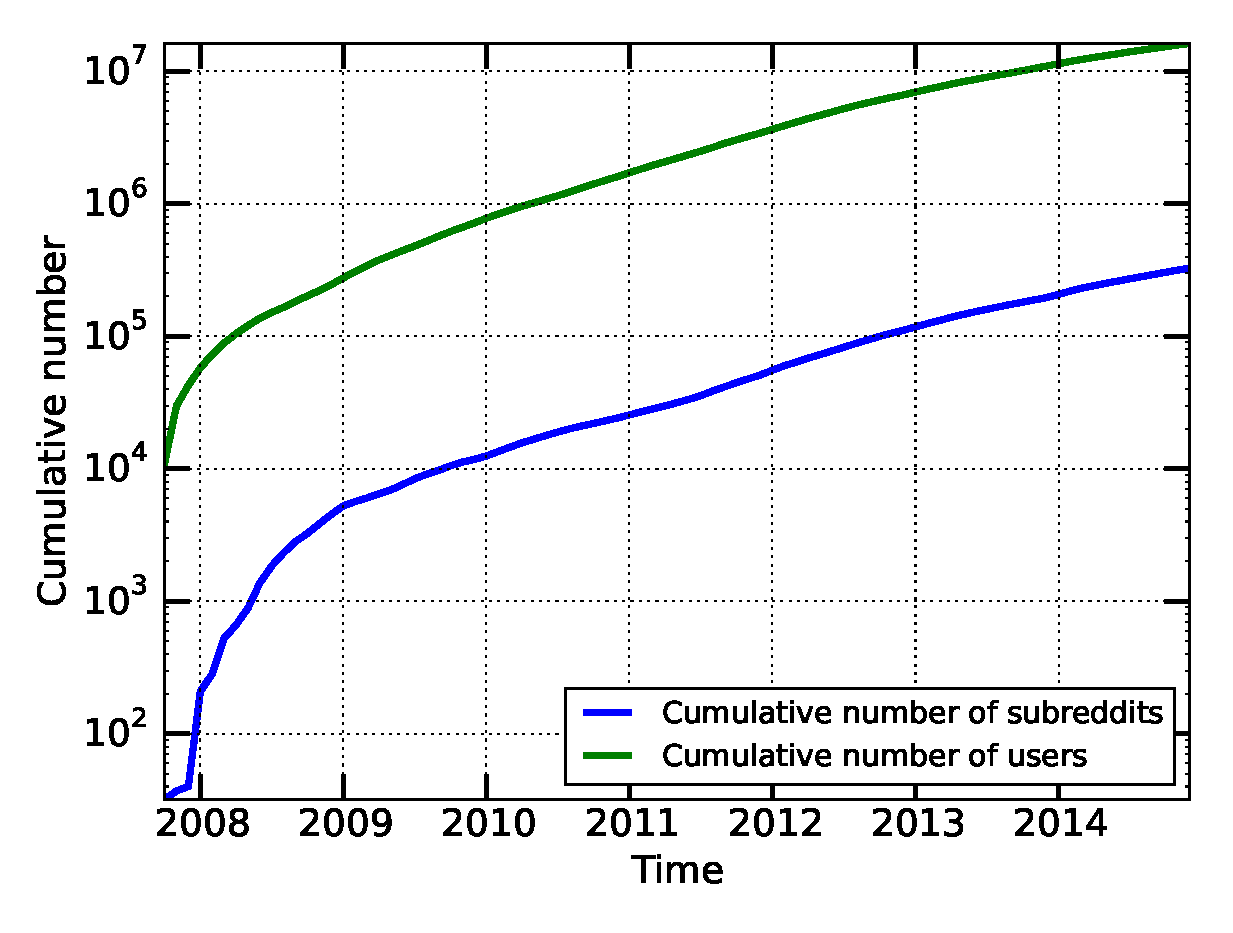
\includegraphics[scale=0.4]{./images/cumulative_users_subreddits.eps}
\caption{Caption}
\label{fig:cumulative_users_subreddits}
\end{figure}

We have identified that about 16.2 million distinct registered users made comments in reddit since its conception until the end of 2014, while around 327 thousand subreddits received comments. 

Since not all users post every month, the cumulative value might not be representative of how many users actually use reddit. If we consider only the users that authored a comment and the subreddits that had comments written at, we have the following graph.

\begin{figure}[!tb]
\centering
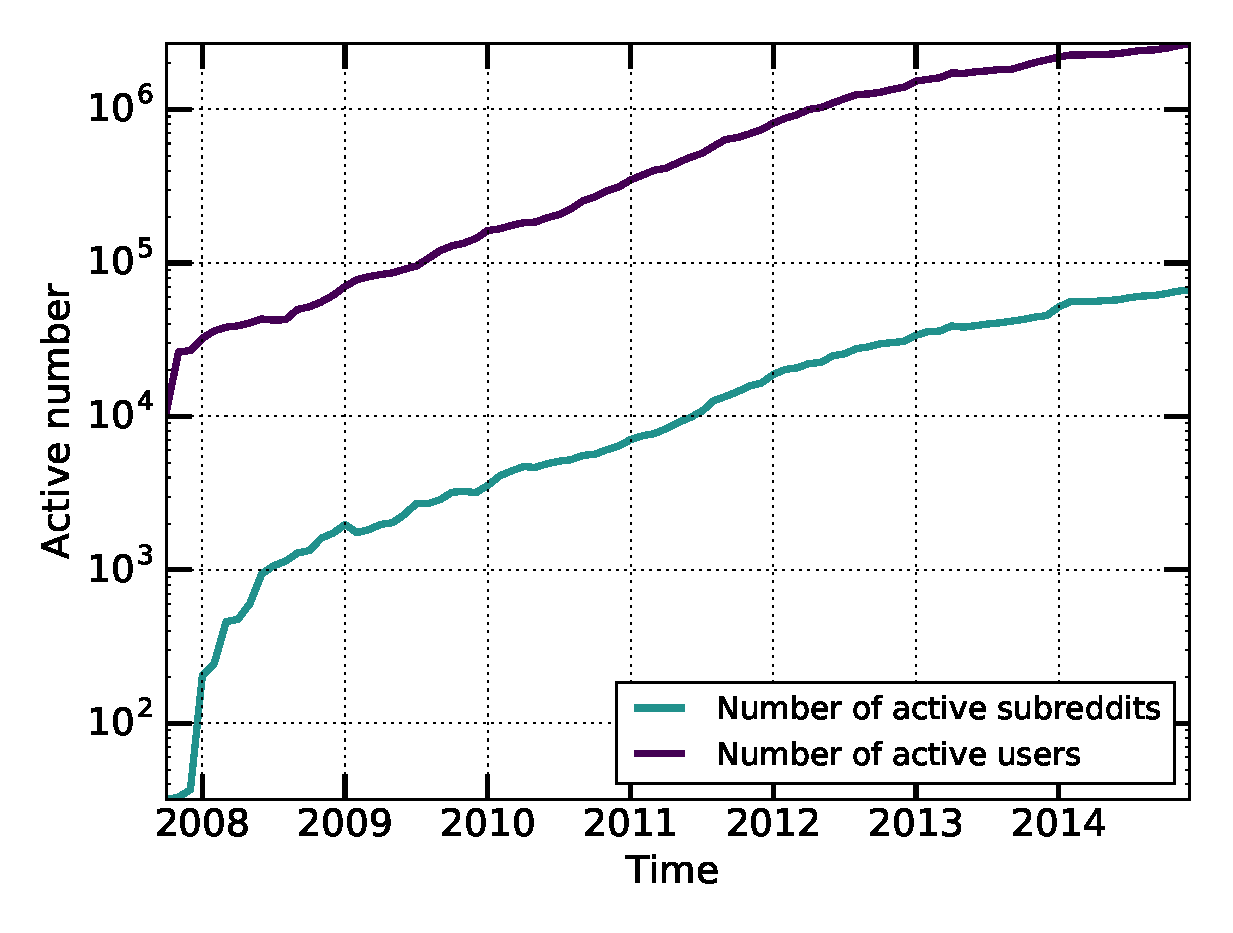
\includegraphics[scale=0.4]{./images/active_users_subreddits.eps}
\caption{Caption}
\label{fig:active_users_subreddits}
\end{figure}

In this graph, we can see that reddit had around 470 thousand users that made comments in the last month of 2014, while around 11400 subreddits received comments in this same month. While the cumulative growth of reddit is impressive, the actual active community is significantly smaller than the total number of existing registered users and subreddits, as expected.

The fact that such a significant amount of users stopped using the platform raises questions such as why users give up on their accounts, when they do so and which users are more likely to stay active. 

\subsection{Identifying cohorts}
%% Amit 9: Added this subsection here. Having the cohorts defined as the part of the overview will help, as we talk about them throughout the paper. Some of the cohort stuff from next section can come here. 
\section{Average posts per user}
In this section, we will use a common metric of user activity in online communities, the number of posts per user over time. Approaches that consider the total number of posts per user in a particular dataset \cite{Gruhl2004} and that analyzes the variation on the number of posts per user over the days \cite{Guo2009} have been applied to online social networks.

\looseness=-1
As we will see, both visualizing behavior relative to a user's join time rather than calendar time and using cohorts provide additional insight into posting activity in Reddit compared to a straightforward aggregate analysis based on clock time.

\subsection{Calendar versus user-relative time}

We start with a common analysis used in this kind of work: aggregating behavior in the community based on calendar time.  Figure~\ref{fig:overall_posts}a shows the average number of posts per month by active users in that month.  Taken at face value, this suggests that over the first few years of Reddit, users became more active in posting, with per-user activity remaining more or less steady since mid-2011.

\looseness=-1

%% Sam 8: Reorganized the next 3 paragraphs, added information about throw away accounts
This average view hides several important aspects of users' activity dynamics. Previous work has looked into behavior relative to the user creation time. It has been shown that edge creation time in a social network relative to the user creation follows an exponential distribution \cite{Tomkins2008}. User lifetime, however, does not follow a exponential distribution and some types of user content generation follow a stretched exponential distribution \cite{Guo2009}. Throw-away accounts are one example of very short-lived users in Reddit \cite{Bergstrom2011}, for example. 

To address these characteristics, Figure~\ref{fig:overall_posts}b shows a different view that emphasizes the trajectory over a user's lifespan. We scale the x-axis not by clock time, as in Figure~\ref{fig:overall_posts}a, but by time since the user's first post: ``1'' on the x-axis refers to one year since the user's account first post, and so on. We call this the \textbf{time in the user referential}. One caution about interpreting graphs with time in the user referential is that the amount of data available rapidly decreases over time as users leave the community, meaning that values toward the right side of an individual data series are more subject to individual variation.  

A tempting conclusion at this point is that the longer a user survives, the more posts they make over time.  This conclusion, however, is incorrect; we will present a more nuanced description of what is happening informed by cohort-based analyses.

\subsection{New cohorts do not catch up}

\begin{figure*}[!tb]
\centering
\subimage[width=0.48, scale=0.42]{./images/avr_posts_per_user_over_time_cohorts.eps}
\subimage[width=0.48, scale=0.42]{./images/avr_posts_per_user_cohorts.eps}
\caption{Figure (a) shows the average number of posts per active users over clock time and Figure (b) the active users in the user-time referential, both segmented by users' cohorts. The user cohort is defined by the year of the user's creation time.  For comparison, the black line in Figure (a) represent the overall average.}
\label{fig:avr_posts_per_user_over_time_cohorts}
\end{figure*}

\looseness=-1
Figure~\ref{fig:overall_posts}b suggests that older users are more active than newer ones, raising the question of whether newer users
will eventually follow in older users' footsteps.  Analyzing users' behavior by cohort is a reasonable way to address this question.

Figure~\ref{fig:avr_posts_per_user_over_time_cohorts}a shows our first attempt at this analysis.  This Figure already shows a significant cohort effect: users from later cohorts appear to level off at a significantly lower posting average than users from earlier cohorts.  It suggests that newer users probably will not ever be as active on average as older ones.

\looseness=-1
However, Figure~\ref{fig:avr_posts_per_user_over_time_cohorts}a also has an awkward anomaly, the rapid rise in the average number of posts during each cohort's first calendar year, especially in December. Combing cohort segmentation with user-referential analysis, as in Figure~\ref{fig:avr_posts_per_user_over_time_cohorts}b, helps smooth out this anomaly and aligns cohorts with each other.  Doing this alignment makes clear that differences between earlier and later cohorts are apparent early on.

\subsection{Does tenure predict activity, or vice versa?}

\begin{figure*}[!tb]
\centering
\subimage[width=0.31, scale=0.29]{./images/avr_posts_per_user_for_surviving_year_for_2010.eps}{2010 cohort}
\subimage[width=0.31, scale=0.29]{./images/avr_posts_per_user_for_surviving_year_for_2011.eps}{2011 cohort}
\subimage[width=0.31, scale=0.29]{./images/avr_posts_per_user_for_surviving_year_for_2012.eps}{2012 cohort}
\caption{Each Figure corresponds to one cohort, from 2010 to 2012, left to right. The users for each cohort are further divided in groups based on how long they survived: users that survived up to 1 year are labeled 0, from 1 to 2 years are labeled 1, and so on.  For all cohorts, longer-tenured users started at higher activity levels than shorter-tenured ones.}
\label{fig:avr_posts_per_user_for_surviving_year}
\end{figure*}

\looseness=-1
These graphs still support the tempting conclusion that users become more active the longer they exist in Reddit, and they do not explain the very rapid increase in posting activity in the first few months.  An alternative hypothesis, inspired by the ``Wikipedians are Born, not Made'' paper \cite{Panciera2009}, is that individual users come in with different posting propensities, and the rise over time is not that individual users become more active but that low-activity users leave the system.  To examine this, we further segment each cohort by the number of years they were active in the system, as defined by the difference between their first and last post times.
 
Figure~\ref{fig:avr_posts_per_user_for_surviving_year} shows this analysis for the 2010, 2011 and 2012 cohorts\footnote{We only show these figures for the sake of saving space, but the same trends are observed in the other cohorts.}.  Across all cohorts and yearly survival sub-cohorts, users who leave earlier come in with a lower initial posting rate.  Thus, the rise in average posts per active user is driven by the fact that users who have high posting averages throughout their lifespan are the ones who are more likely to survive.  As the less active users leave the system, the average per active user increases.  In other words, the correct interpretation of Figure~\ref{fig:overall_posts}b isn't that longer-lived users post more.  It actually is that users who post more---right from the beginning---live longer. 

Combining Figure~\ref{fig:avr_posts_per_user_for_surviving_year}'s insight that the main reason why these curves increase is because the low posting users are dying sooner with the earlier observation that the stable activity level is lower for newer cohorts suggests that low-activity users from later cohorts tend to survive longer than those from earlier cohorts.  That is, people joining later in the community's life are less likely to be either committed users or leave than those from earlier on: they are more likely to be ``casual'' users that stick around.

\vspace{7pt} 
\section{Comment length}

\begin{figure*}[!tb]
\centering
\subimage[width=0.48, scale=0.42]{./images/avr_comment_size_over_time_cohorts.eps}
\subimage[width=0.48, scale=0.42]{./images/avr_comment_size_cohorts.eps}
\subimage[width=0.31, scale=0.29]{./images/avr_comment_length_for_surviving_year_for_2010.eps}{2010 cohort}
\subimage[width=0.31, scale=0.29]{./images/avr_comment_length_for_surviving_year_for_2011.eps}{2011 cohort}
\subimage[width=0.31, scale=0.29]{./images/avr_comment_length_for_surviving_year_for_2012.eps}{2012 cohort}
\caption{Figure (a) shows the average comment length over clock time and Figure (b) from the user-referential time. Both figures show the cohorted trends.  The overall average length per comment decreases over time, although for any individual cohort, it increases after a sharp initial drop. Figures (c), (d) and (e), similar to Figure~\ref{fig:avr_posts_per_user_for_surviving_year}, shows the monthly average comment length for active users in the cohorts of 2010, 2011 and 2012, segmented by the number of years that the user survived in the network.  Opposite the analysis for average posts, which showed that low-activity users were the first to leave Reddit, here, people who start out as longer commenters are \textit{more} likely to leave.}
\label{fig:comment_length}
\end{figure*}

Activity as measured by the average number of posts per user is one proxy for user effort.  Comment length can also be considered as a proxy for user effort in the network.  Users that type more put more of their time in the network, contribute with more content, and might create stronger ties with the community.  Thus, we investigate how comment length has changed in the community over time, both overall and by cohort. 

\subsection{Comment length drops over time}

Figure~\ref{fig:comment_length}a shows the overall comment length in Reddit over time (the black line) and the overall length per cohort. 
Based on the downwards tendency of the overall comment length in Figure~\ref{fig:comment_length}a, one might infer that users' commitment to the network is decreasing over time, or that there is some community-wide norm toward shorter commenting. 

This, however, might not be the best way to interpret this information. Figure~\ref{fig:comment_length}b shows the comment length per cohort based on the user referential time. An important thing to notice here is that younger users start from a lower baseline comment length than older users. Together with the fact that recent Reddit has experienced exponential growth, the weight when evaluating the overall average for Figures \ref{fig:comment_length}a and \ref{fig:comment_length}b is shifted towards the comment length for the ever-growing younger generation as the years go by; this younger generation brings the average down since they write less on average.

\subsection{Simpson's Paradox: the length also rises}

Let us go back to Figure~\ref{fig:comment_length}a, which shows the overall average comment length on Reddit over time. We see a clear trend towards declining length of comments in the overall line (the black line that averages across all users). This could be a warning sign for Reddit community managers, assuming longer comments are associated with more involved users and healthier discussions. A data analyst looking at these numbers might think about ways to promote longer comments on Reddit. 

However, in Figure~\ref{fig:comment_length}b, we saw that average comment length increases over time for every cohort. While later cohorts start at smaller comment length, after an initial drop, all cohorts show positive trends towards writing longer comments over time.  This is puzzling: when each of the cohorts exhibits a steady increase in their average comment length, how can the overall mean comment length decrease?  This anomaly is an instance of the Simpson's paradox \cite{simpson1951}, and occurs because we fail to properly condition on different cohorts when computing mean comment length. 

\begin{table}[!tb]
\centering
\tabcolsep=0.07cm
\singlespacing
\fontsize{9pt}{10.5pt}\selectfont
\begin{tabular}{|c|c|c|c|c|c|c|c|c|c|}
\cline{2-9}
\multicolumn{1}{c|}{} & \multicolumn{8}{c|}{Cohorts} \\ \hline
Year & 2007 & 2008 & 2009 & 2010 & 2011 & 2012 & 2013 & 2014 & Overall\\ \hline
2007 & 220 & - & - & - & - & - & - & - & 220 \\ \hline
2008 & 208 & 198 & - & - & - & - & - & - & 204 \\ \hline
2009 & 224 & 204 & 201 & - & - & - & - & - & 208 \\ \hline
2010 & 223 & 204 & 189 & 184 & - & - & - & - & 193 \\ \hline
2011 & 233 & 211 & 199 & 184 & 167 & - & - & - & 182 \\ \hline
2012 & 241 & 221 & 212 & 197 & 173 & 167 & - & - & 178 \\ \hline
2013 & 244 & 225 & 214 & 199 & 177 & 167 & 164 & - & 174 \\ \hline
2014 & 246 & 229 & 217 & 204 & 183 & 172 & 165 & 176 & 176 \\ \hline
\end{tabular}
\caption{Evolution of the average throughout the years for each cohort. Each column here is one cohort and each line is one year in time. Cohorts only start having data on the cohort year, therefore the upper diagonal is blank. On the right column we see the overall average for all users.}
\label{tab:simpson}
\end{table}

Table~\ref{tab:simpson} provides some clues to what might be going on. When we move down the rows, we observe an increasing tendency in each cohort column. It means that the average comment length increases for these users. However, when we move right through the columns, people in later cohorts tend to write less per comment. If we were to average each row, we would still get an overall increasing comment length per year, but that is not what we see in the overall column. What happens here is that the latter cohorts have many more users than earlier ones. Since their numbers increase year by year, we have a much larger contribution from them towards comments, compared to users of earlier cohorts. This uneven contribution leads to the paradox we observed in Figure~\ref{fig:comment_length}a. 

Without the decision to condition on cohorts, one would have gathered an entirely wrong conclusion. People are not writing less as they survive, rather those who tend to write less are joining the community in much larger numbers. Knowing this, one may focus on better onboarding processes for newcomers, or try to learn why users in later cohorts tend to write smaller comments on average.  

\begin{figure*}[!tb]
\centering
\subimage[width=0.48, scale=0.42]{./images/comments_per_submissions_over_time_cohorts.eps}
\subimage[width=0.48, scale=0.42]{./images/comments_per_submissions_cohorts.eps}
\subimage[width=0.23, scale=0.23]{./images/comments_per_submissions_for_surviving_year_for_2008.eps}{2008 cohort}
\subimage[width=0.23, scale=0.23]{./images/comments_per_submissions_for_surviving_year_for_2009.eps}{2009 cohort}
\subimage[width=0.23, scale=0.23]{./images/comments_per_submissions_for_surviving_year_for_2010.eps}{2010 cohort}
\subimage[width=0.23, scale=0.23]{./images/comments_per_submissions_for_surviving_year_for_2011.eps}{2011 cohort}
\caption{Figure (a) shows the average comment per submission ratio over clock time for the cohorts and the overall average. Figure (b) shows the average comment per submission from the user-referential time for the cohorts. Figures (c), (d), (e) and (f), similarly to Figure~\ref{fig:avr_posts_per_user_for_surviving_year}, shows the 2008, 2009, 2010, and 2011 cohorts, segmented by the number of years a user in the cohort survived.  As with average posts per month, users who stay active longer appear to start their careers with a relatively higher comments per submission ratio than users who abandon Reddit sooner.  Unlike that analysis, however, the early 2008 cohort ends up below the later cohorts in Figure (b).}
\label{fig:comments_submissions}
\end{figure*}

\subsection{New users burn brighter}
As with the posting per user, we can not say if the increase in the curves seen in \ref{fig:comment_length}b are due to the lower effort users dying first or because users are writing more as they live on the network. To answer this, \ref{fig:comment_length}c allow us to make two important observations: first, \textit{comment length does increase inside of each cohort}, no matter how long the user survives. Secondly, as a general trend, \textit{users that make longer comments inside of each cohort die faster}. This is quite surprising, given that we would expect people to put less effort when they are more likely to stop using the network.

\section{Kinds of contributions}

One common question from the literature is what sorts of activities users engage in, for instance, to categorize users into roles they play in the community\cite{Welser2011}.

\subsection{Over time, responsiveness increases}
Consider the case of Usenet: people who never start threads and only respond play the role of answerer, while there are other roles that include fostering discussion \cite{Welser2007}. These might naturally map onto people who primarily comment and who primarily submit in Reddit, respectively.  While submissions can be considered new content that an author generates, a comment can be considered as a contribution to an existing content from another author.

Since the total number of comments always surpasses the number of submissions, Figure~\ref{fig:comments_submissions}a shows the evolution of the overall and cohorted ratio of the average number of comments a user makes for each submission they make over time from 2008 until 2013. Here we see that users who most prefer commenting to submitting come from 2009, 2010 and 2011, and we observe that, over time, the average ratio of comments to submissions increases both overall and per-cohort for active users.

Again, we analyze our data from the user-time referential, as seen in Figure~\ref{fig:comments_submissions}b. It shows a clear pattern for users in earlier cohorts to have a lower comment per submission ratio than users in later cohorts ones, given that they both survived the same amount of time.  Surviving users from later cohorts also exhibit a more rapid increase in comments per submission than those from earlier cohorts.  In particular, the 2008 and 2009 cohorts increase much more slowly over time than those from 2010 onwards; later cohorts are more similar (although the 2012 and 2013 cohorts may level off lower than 2011 based on the limited data we have). 

\subsection{Comment early, comment often}

Figure~\ref{fig:comments_submissions}c shows the cohorts from 2008, 2009, 2010 and 2011 segmented by surviving year.  Three interesting observations arise from these data.  First, we see that just as in the analysis of average posts per user, the users who survive the longest in each cohort are also the ones who hit the ground running.  They start out with a high comment-to-submission ratio relative to users in their cohort who abandon Reddit more quickly.  This suggests that both the count of posts and the propensity to comment might be a strong predictor of user survival.

Second, and unlike the case for average post length, surviving users' behavior changes over time.  Figure~\ref{fig:avr_posts_per_user_for_surviving_year} shows that even for the most active users, they come in at a certain activity level and stay there, perhaps even slowly declining over time.  Here, the ratio of comments to submissions increases over time; combined with the observation that overall activity stays steady, this suggests that the ratio is changing because people \textit{substitute} making their own submissions for commenting on others' posts.

Finally, this increase is most pronounced for the earliest cohorts from 2008 and 2009, with ratios more than doubling over their first year, much more than the change for later cohorts.  Still, the ratio for these earlier cohorts never rises to the level it does for surviving users from later cohorts. 

%%% DC 12: Moving this as part of the section on comment length.
%% DC 12: I think subreddits and joint_cohorts probably get merged since they're largely explained by the same phenomenon of default subreddits for new users.
%\section{Subreddits}

\subsection{Subreddits Activity}

One way to look at reddit is as a multi-community social network. Each subreddit can be considered as a semi-independent community, and as such, we can study the evolution of these communities based on time, cohorts and survivability.  A number of other online communities have similar properties, with tighter (Wikiprojects, enterprise social network discussion groups) or looser (Wikia, StackOverflow) interdependence between the individual sub-communities.

One of the initial question we can ask is how is the number of posts in these surviving communities evolving? One thing to be aware here though is that this variable is likely to be sensitive to the ration of active users per active subreddits. If we imagine that users don't change their posting patterns rapidly, and increased number of users per subreddits implies in an increased number of posts per subreddit. The overall number of users per subreddits, however, seems fairly stable throughout the years.

Figure N shows the evolution of number of posts per active subreddits in time for subreddits created between 2008 and 2013. We can observe that the average number of posts per subreddit increases over time. Since the ratio of active users per subreddit remains relatively stable, one could imagine that subreddits are receiving more posts throughout the time.

\begin{figure}[!tb]
\centering
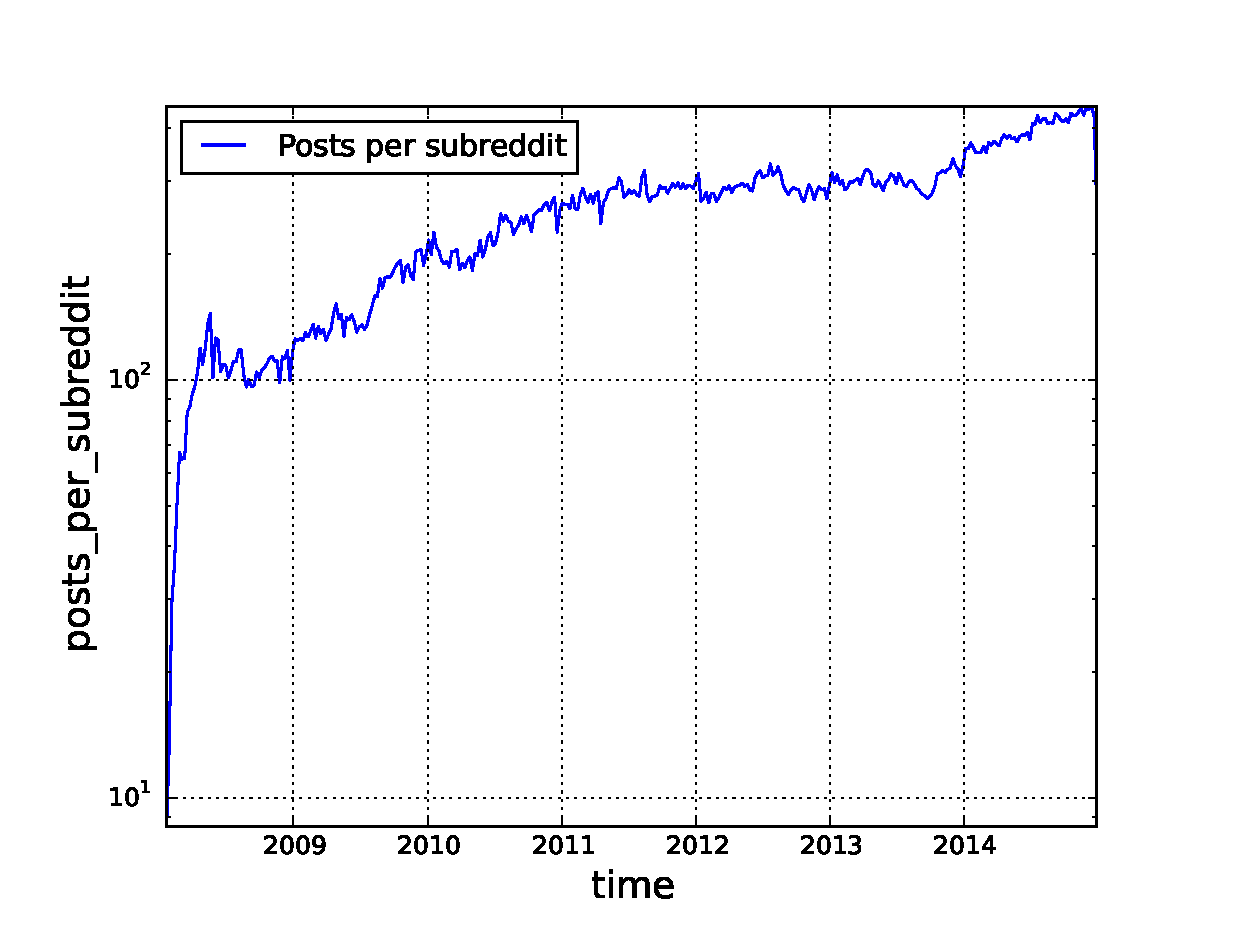
\includegraphics[scale=0.4]{./images/posts_per_subreddit_over_time_total.eps}
\caption{Caption}
\label{fig:posts_per_subreddit_over_time_total}
\end{figure}

To better understand how correct is this conclusion, we cohort the subreddits in time. We can observe that the majority of posts in reddit are made in 2008 subreddits, and the posting averages for this cohort dominates the total posting average for the whole social network. Also, we notice that for most points in time, the number of posts per subreddits increases as we move to older cohorts. This, however, is not sufficient for us to conclude that these communities are evolving in different ways, since subreddits from older cohorts had more time to consolidate their reach and popularity and most of the ``likely to die'' subreddits that bring the average number of posts down in newer cohorts are still alive.

\begin{figure}[!tb]
\centering
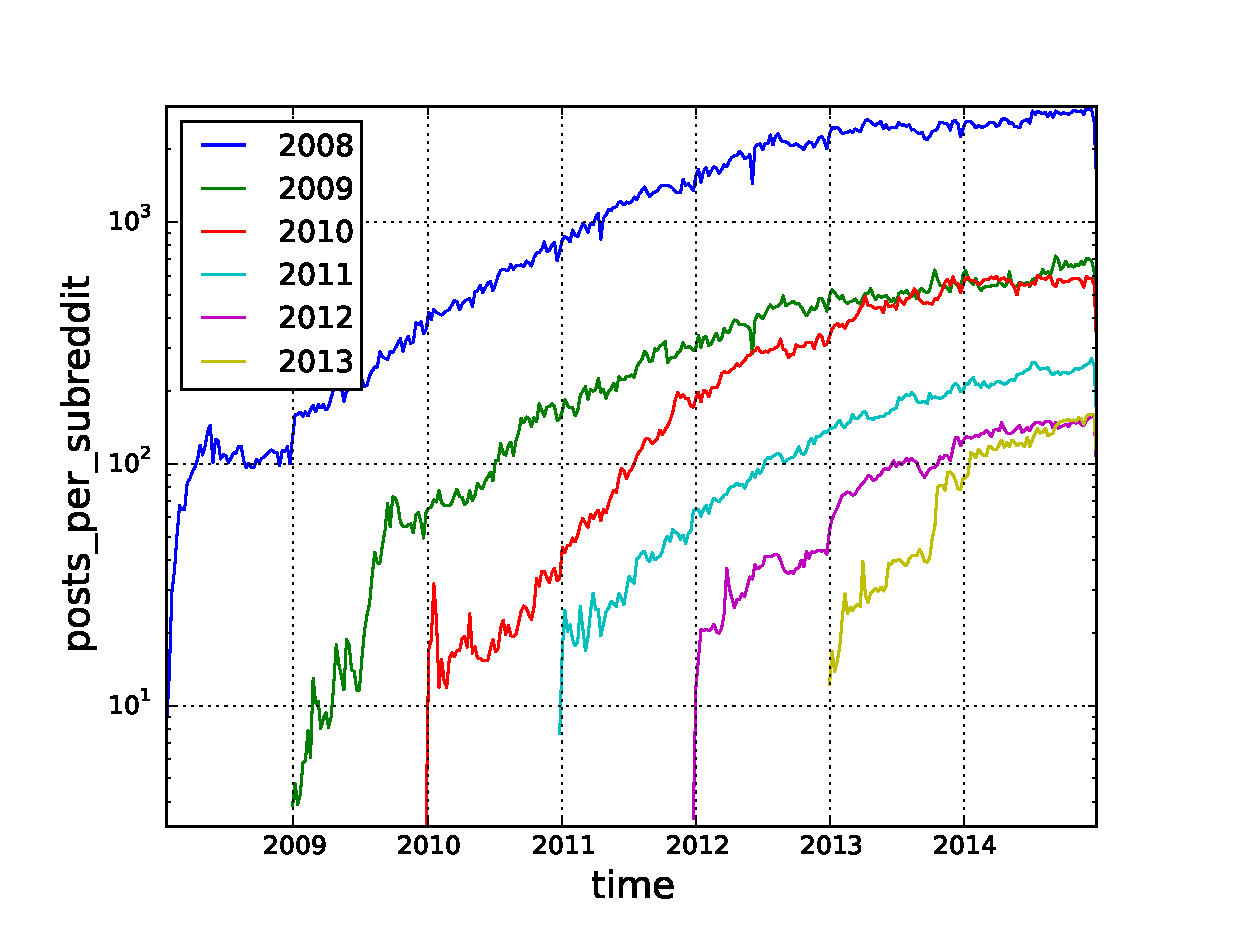
\includegraphics[scale=0.4]{./images/posts_per_subreddit_over_time_cohorts.eps}
\caption{Caption}
\label{fig:posts_per_subreddit_over_time_cohorts}
\end{figure}

To properly compare these communities starting from the same baseline, we evaluate every posting time according to the subreddit creation time (fists post ever made in the subreddit). The x-axis then becomes the time the subreddit has lived, grouped by cohort. This approach reveals a general trend of subreddits from newer cohorts stabilizing in a lower posting average than older cohorts. This, however, does not hold true for the 2009 and 2010 cohorts, although they stabilize in very similar levels, and for the 2013 cohort, for which we have only one year of data in the overlap for all subreddits.

\begin{figure}[!tb]
\centering
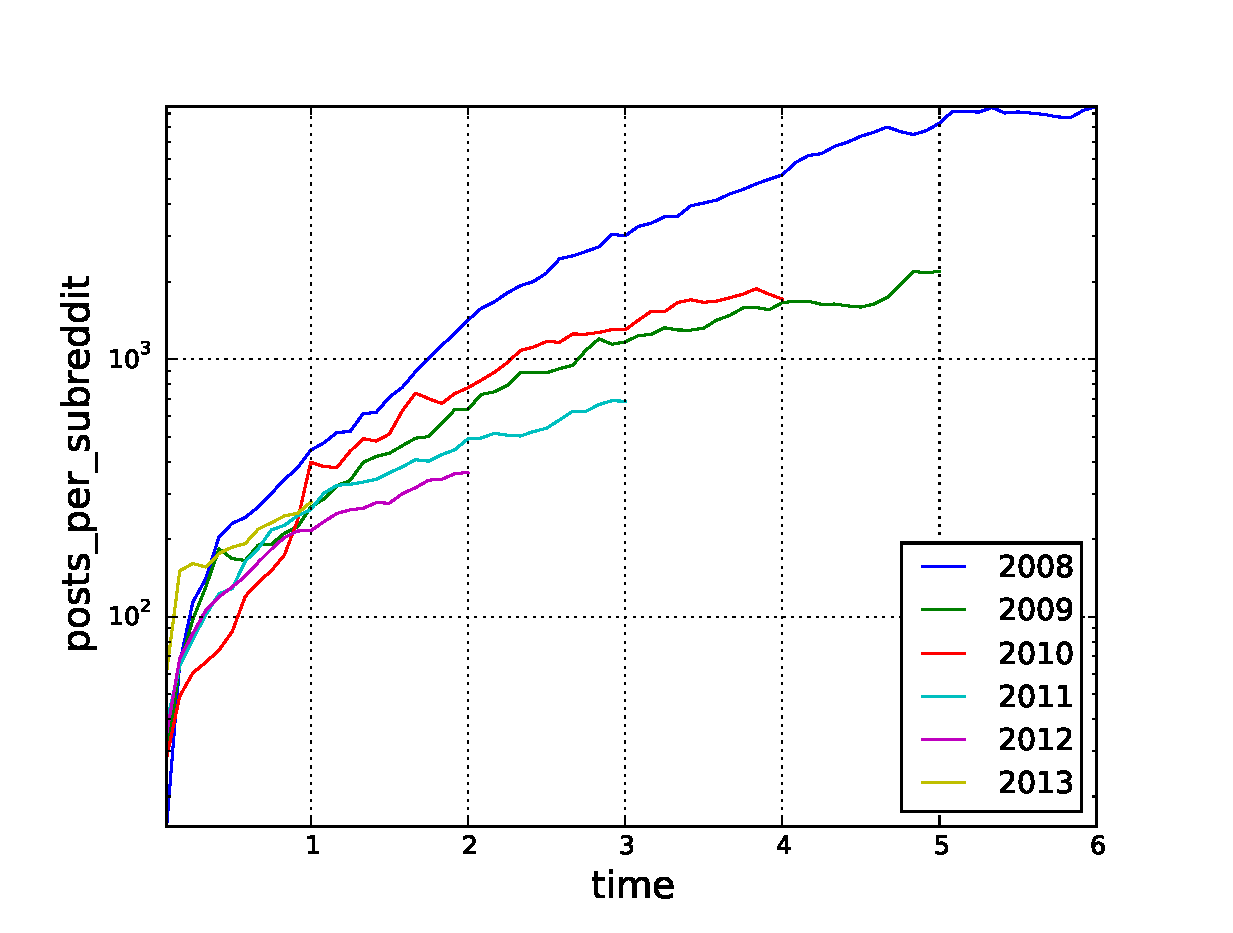
\includegraphics[scale=0.4]{./images/posts_per_subreddit_cohorts.eps}
\caption{Caption}
\label{fig:posts_per_subreddit_cohorts}
\end{figure}

Assuming that subreddits that survive have, on average, a higher number of posts than the ones that do not survive, part of the higher levels of posting for the older cohorts could also be explained by a faster ``death rate'' of the low posting subreddits. Therefore, the faster the number of posts per subreddit grows, the faster the non-fit subreddits are being eliminated.

\subsection{Subreddits' Survival}

Similarly to what we did for users, we look in a one year time window for the last post that was created for each subreddit and define as subreddits that died as the ones that the last post happened in the first nine months of the one year window. The Kaplan-Meier curve is shown in Figure N.

\begin{figure}[!tb]
\centering
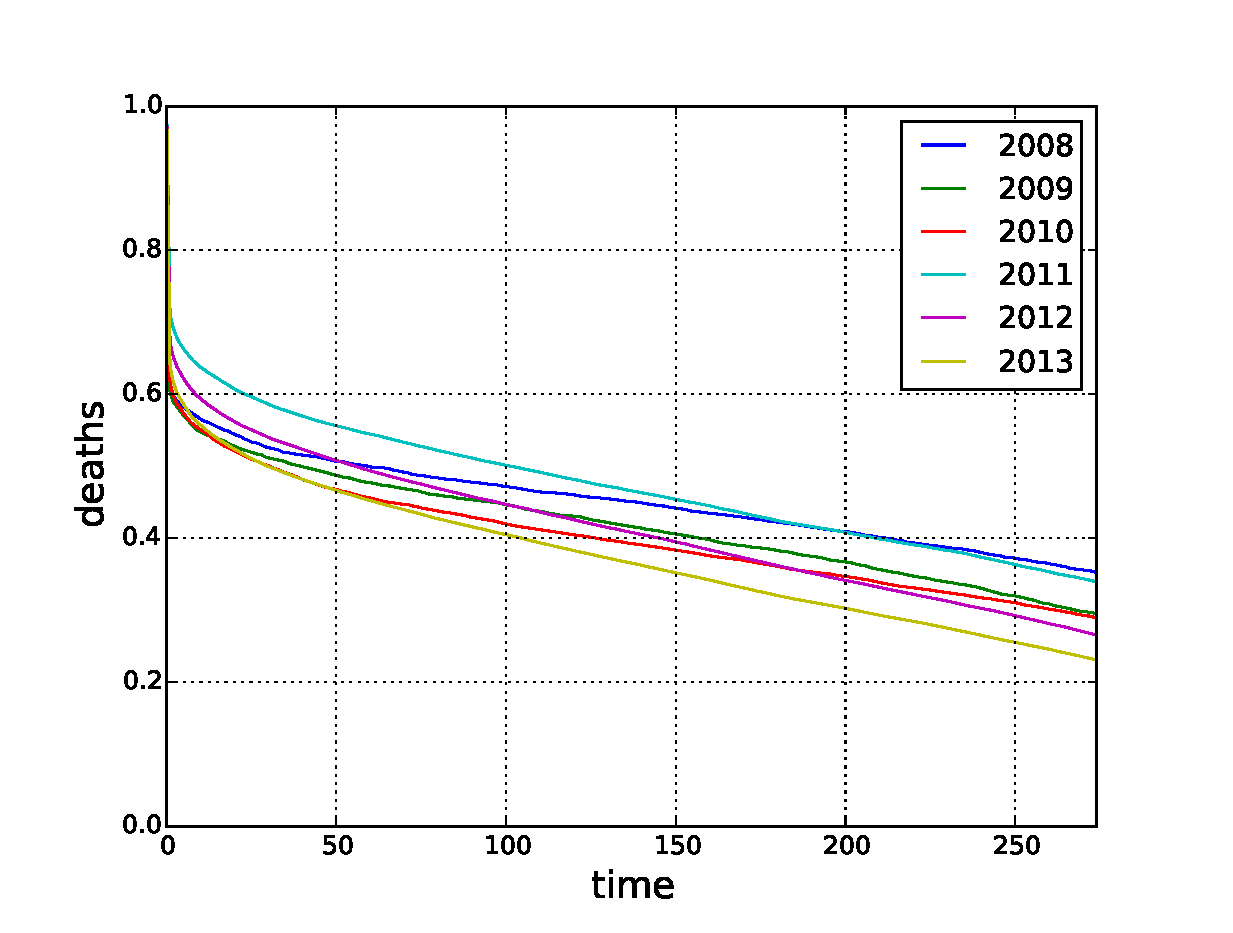
\includegraphics[scale=0.4]{./images/kaplan_meier_subreddits.eps}
\caption{Caption}
\label{fig:kaplan_meier_subreddits}
\end{figure}

In this survival curve, we also observe that there is a significant number of subreddits that survive only through the first day, just as seen with the users, although the proportion in this case is not as high as the users . Also, unlike the users, there are significantly differences in the ``decay of subreddits''.

\begin{figure}[!tb]
\centering
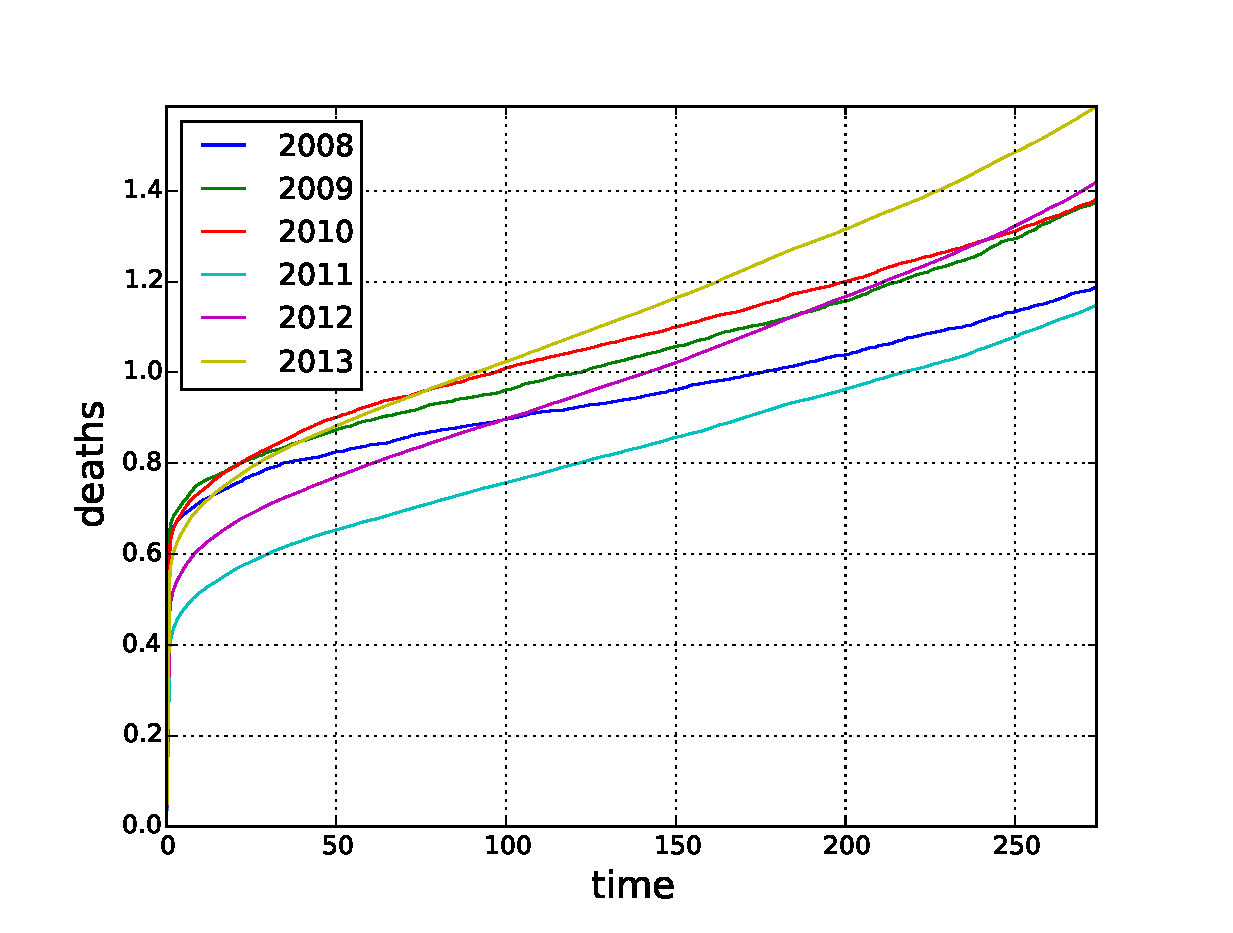
\includegraphics[scale=0.4]{./images/nelson_aalen_subreddits.eps}
\caption{Caption}
\label{fig:nelson_aalen_subreddits}
\end{figure}
\section{User Bias for Early Content}

\begin{figure*}[!tb]
\centering
\begin{subfigure}{.3\textwidth}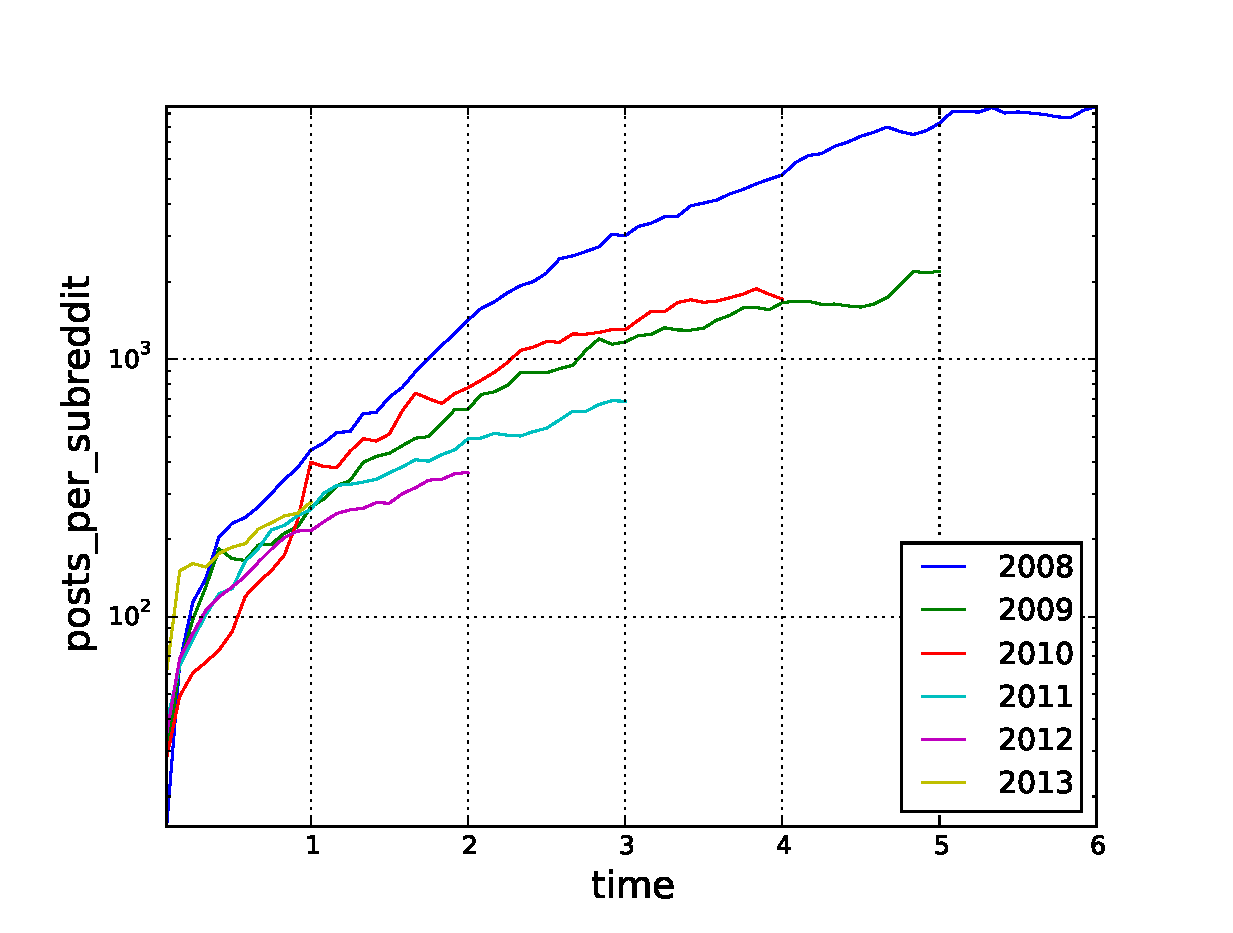
\includegraphics[scale=0.285]{./images/posts_per_subreddit_cohorts.eps}\caption{}\end{subfigure}
\begin{subfigure}{.3\textwidth}\includegraphics[scale=0.285]{./images/user_subreddit_submissions_cohorts.eps}\caption{}\end{subfigure}
\begin{subfigure}{.3\textwidth}\includegraphics[scale=0.285]{./images/user_subreddit_comments_cohorts.eps}\caption{}\end{subfigure}
\caption{Caption}
\label{fig:user_subreddit_submissions_cohorts}
\end{figure*}

The cohort a user belongs to has a significant impact to the user posting behavior, but that does not give us a picture of how these users coexist in the current community. An interesting hypothesis that we could imagine is that users from a particular cohort are more interest in the communities from a particular cohort. We now look at the interplay between user and subreddit cohorts. 

An initial hypothesis would be that users would be interested in the communities that were being created at the same time they joined the network. To test for that, Figures N and N show the number of submissions and comments per user, respectively, based on the user and subreddit cohorts.

It is possible to see that users' behavior, independently of the cohort, are biased to subreddits created on 2008. 2008 users' submissions are particularly more biased to 2008 subreddits. This might be due to the fact that these surviving users play a much more central role in these communities (moderators or key contributors) since they are more likely to be there from the start.

These observations allow us to conclude that, in the case of reddit, there are key subreddits that were created in 2008 that are the main focus of attention of all the users, although this is decreasing as new users join the network. Our hypothesis would not hold true in this case. This, however, might not hold true for other social networks, in which the communities or the content at the time at which users join the network might be their main focus of attention, highlighting again the importance of performing a cohort based analysis.

\section{Discussion}

In this section we discuss some of the processes that might explain our observations and refer to the associated literature. We're not taking a position on either of these as the mechanism that explains these results; both would be interesting avenues for future work.  We do suggest that looking at Reddit from a cohort and user-based view rather than an aggregate community view helped us uncover interesting phenomena and questions that would have been invisible to more commonly-performed analyses of community behavior. 

% Sam 12: Took if from the users' posting section to here. We should probably rethink this.
\subsection{Why more low activity users are surviving?}

%% DC 10: The status bit is intriguing but needs to be explained a little better.  Took a little shot at it but framing it in terms of cumulative advantage rather than status
%% DC 10:This, too, would need to be explained/justified/supported, and I can't come up with a plausible one, so deleting it.
%Yet another explanation would be that earlier users demographics were different in terms of age and interests, for example, and these correlate to the fact that they present a higher activity.
We have seen that users from latter cohorts have a lower posting average than in earlier cohorts. It has been shown that online book reviews have a self-selection problem, since early reviews tend to be positively biased \cite{Li2008}. 
%% Sam 14: Found one talking about books in amazon, they call it a self-selection bias problem
%, in the same way that early ratings for a movie in a recommender system are likely to be higher than later ratings because the people who are most attuned to the movie are likely to see it earlier \cite{if_we_can_find_one}.
One plausible explanation is that users who find a community early in its life are also more likely than average to be those who will be attracted to it. This would mean that the mixture of users joining in the early stage of the community are more likely to be the most active ones and the latter ones are more likely to be less active. A higher number of less active users joining the network would also account for their longer survival, although other mechanisms might also be in play.

Another is an argument based on cumulative advantage, status, and attention-seeking: surviving users from earlier cohorts might be more capable of producing content that gets attention from other users.  This would lead to them getting more comments and votes for their content, and people who get positive attention are more likely to return \cite{Halfaker2009, Choi2010, Sarkar2012}.  

\subsection{Why are comments getting shorter?}

One hypothesis that we might consider to explain the decreasing comment length of the users is associated to an ``initial value problem''. We can imagine that users, as they join the network, tend to produce content according to the norms of what they see \cite{Kooti2010, Danescu-niculescu-mizil2013}. The observed behavior of the comments length for the users in reddit is a initial drop, followed by steady increase as the user survives. If the starting point for the initial drops are taken as the average of the network, that is what is observed by the user in the network, the initial drop would place each cohort starting at lower levels than the previous one.

\subsection{Why comments per submissions are increasing?}

The majority of users in social networks are known to be lurkers: users that only seek information and passively observe, not engaging and contributing to the network \cite{Rafaeli2004, Nonnecke2000}. It is reasonable to expect the same from reddit. On the other hand, social networks often have a small number of ``power contributors''\ref{Panciera2009, Kittur2007}.

When we consider the evolution of the number of comments per submission, we observer a decreasing trend for the older cohorts. Just as lurkers are the majority in the community and are attracted to it in search of information, we can imagine a set of users that are in the community in search of content and is whiling to engage in commenting, but hardly has the drive of a ``power contributor'' to bring new content into the network. Since in early reddit the amount of existing submissions was significant smaller than in the next few years, limited space existed for information seeking lurkers and ``commenters''. As the community grew, more content from an absolute point of view was present in the social network, therefore activities of information seek became more prominent and could explain the increase in commenting activity. 

\subsection{Why the bias to 2008?}

Were we expecting different results? Defaults? Core consolidation? 
These observations allow us to conclude that, in the case of reddit, there are key subreddits that were created in 2008 that are the main focus of attention of all the users, although this is decreasing as new users join the network. Our hypothesis would not hold true in this case. This, however, might not hold true for other social networks, in which the communities or the content at the time at which users join the network might be their main focus of attention, highlighting again the importance of performing a cohort based analysis.

\section{Conclusions}

This work addresses some aspects of how to analyze the evolution of a social network and how to apply and avoid some pitfalls of cohort analysis. To do so, we analyse the reddit network and provide insights on the users posting behavior evolution, we identify a general tendency of newer users to write smaller comments and we discuss user survival from empirical standpoint. 

We also analyse subreddits evolution, considering the volume of activity, how commenting and submitting change in function of cohorts and the matter of community survival as subreddits can be seen as independent communities.

	\section{Future Work}

Although many observations were made regarding reddit, the main goal of this paper is not to study reddit in depth. Therefore, many observations still remain without an explanation. Being aware that users decrease the size of their comments and tend to submit more than comment allow us to question ourselves about the nature and motivation of these users. Are users commenting less because newer users they are less interested into engaging into existing submissions or are they simply ``lazier'' and writing is becoming less attractive for the newer generations? If it is a matter of writing being a less prefered method of communication, could reddit improve its users' interactions providing alternative ways to post media, such as pictures, sound and videos? Regarding subreddits, why are newer subreddits more likely to die? Is it because they can not compete with larger subreddits? Or is it because they are not in direct competition, but they cover a smaller and more niche like space of interests that make it less popular and more likely to die? Or it might just be that their creators from are from newer cohorts and, just as they are ``lazier'' to write, they can not keep up with maintaining their new communities?

These are some questions that we can ask and needs further investigation of the data, and might evolve into new models of how communities compete for spaces of interests or how user attention, effort and interaction in social networks are shifting through time.

One interesting question that recurrently arises when we were performing survival analysis was regarding the users' ``breaks'' from the network. As ``death'' in a social network is not well defined - users can delete their account, which is a clear sign of death, but they can also simple stop using the network - using the last posting date and setting thresholds for activity to be considered alive might not be enough. A next step would be to investigate better definitions of ``death'' and study different types of user behavior to characterize the burstiness of their behavior. Some users might only interact with the network in some specific occasions while some users might have a much more uniform pattern. Understanding how your network fare in terms of user burstiness is essential to understand how the users use the network and to set goals to improve or change the user experience. Also, a better definition of ``death'' would allow us to investigate the ``rebirth'' of users, that is, users that come back to the network. Whereas here we consider it as a right censorship problem, it might pose a much more central issue, as network survival might not only depend only in the ability to attract and retain users, but also in the ability to restore old users.

%% DC 10: This gets moved to discussion/future work, I think.
%% As with many analyses that focus on visible behavior, ours discounts lurkers despite their known importance as audience members \cite{} and future contrtibutors \cite{}.  Many lurkers likely vote, and thus may be even more important in a context like Reddit where votes affect content visibilty and provide explicit markers of attention and reputation.  However, the dataset does not have information on individual voters or timestamps, just the aggregate number of votes a post had received at the time of the crawl, making it impossible to effectively treat them as activity measures and ways to understand the behavior of those who voted.  The voting data might be much more useful, however, in questions that involve predicting a given user's future behavior based on whether and how other users respond to a user's early contributions \cite{joyce_kraut_2006, lampe_everything2, etc.}



\section{Acknowledgments}
The authors are grateful to FAPESP grant \#2011/50761-2, CAPES grant \#99999.009323/2014-07, NAP eScience - PRP - USP, and RepNerv foundation for ongoing support.


\bibliographystyle{abbrv}
\bibliography{bibtex}

\end{document}
